%
% File acl2016.tex
%
%% Based on the style files for ACL-2015, with some improvements
%%  taken from the NAACL-2016 style
%% Based on the style files for ACL-2014, which were, in turn,
%% Based on the style files for ACL-2013, which were, in turn,
%% Based on the style files for ACL-2012, which were, in turn,
%% based on the style files for ACL-2011, which were, in turn, 
%% based on the style files for ACL-2010, which were, in turn, 
%% based on the style files for ACL-IJCNLP-2009, which were, in turn,
%% based on the style files for EACL-2009 and IJCNLP-2008...

%% Based on the style files for EACL 2006 by 
%%e.agirre@ehu.es or Sergi.Balari@uab.es
%% and that of ACL 08 by Joakim Nivre and Noah Smith

\documentclass[11pt]{article}
\usepackage{acl2016}
\usepackage{times}
\usepackage{url}
\usepackage{latexsym}
\usepackage{xcolor}
\usepackage{latexsym}
\usepackage{tabularx} 
\usepackage[english]{babel}
\usepackage{multirow}
\usepackage{booktabs}
\usepackage{ifthen}
\usepackage{tikz,pgfplots}
\usepackage{xcolor,colortbl}
\usepackage[color=cyan]{todonotes}
\usepackage{tikz}
\usepackage{pgfplots}
\usepackage{fancybox}
\usepackage[normalem]{ulem}
\useunder{\uline}{\ul}{}

\newcommand{\tnumb}[1]{\fontfamily{phv}\selectfont #1}%

\newcommand{\DEVELOPMENT}{1} % 1= show comments, 0=no comments
\usepackage{ifthen}
\ifthenelse{\DEVELOPMENT = 1}{
	\newcommand{\tz}[1]{\textcolor{cyan}{\textbf{TZ:} #1}}		
	\newcommand{\mw}[1]{\textcolor{red}{\textbf{MW:} #1}}				
}{
	\newcommand{\tz}[1]{}		
	\newcommand{\mw}[1]{}			
}


%\aclfinalcopy % Uncomment this line for the final submission
%\def\aclpaperid{***} %  Enter the acl Paper ID here

\setlength\titlebox{4cm}
% You can expand the titlebox if you need extra space
% to show all the authors. Please do not make the titlebox
% smaller than 5cm (the original size); we will check this
% in the camera-ready version and ask you to change it back.

\newcommand\BibTeX{B{\sc ib}\TeX}

\title{Status Report}

\author{Michael Wojatzki}

\date{}

\begin{document}
\maketitle
\begin{abstract}
This document gives an overview on the progress of my PhD and covers the following aspects:
First, I briefly outline theoretical background and important assumptions of the project. 
Thereby, I will discuss current state of our knowledge and do not reflect how it has developed over time.
Second, I describe a methodological framework in which we can arrange the conducted research.
As I mainly work data-driven this section focusses on data.
While this framework does not completely fit all of the conducted research, I try to be as comprehensive as possible.
Using this framework, I subsequently reflect on results which are obtained in the so far executed experiments.
As requested by the last reviews, I will thereby clearly differentiate between published, unpublished but finished and unfinished works. 
Finally, this report closes with remarks regarding future work and on professional activities such as networking and organized workshops.

\end{abstract}

\section{Introduction}

In my PhD project I am dealing with the automatic analysis of discussions and debates conducted on social media platforms.
Besides developing and improving algorithms that are capable of detecting arguments, positions, substantiations, etc., goal of the project is to utilize these algorithms to contribute to a better understanding of social media discussions.
Being capable of automatically analyzing social media discussions aids a huge variety of practical applications for information seekers such as researchers, journalists, customers, users, companies, or governments.
In addition, such analysis could help to create summaries, develop a deeper understanding of online debating behavior, identify social or political groups, or even adjust recommendations to users' standpoints \cite{anand2011cats,sridhar2014collective,boltuzic2014back}.

My work is located at the interface between different strands from the research field of natural language processing or computational linguistics.
The first strand is called is called \textit{Argument Mining} and is concerned with the identification of argumentative structures within written communication \cite{green2014argmining}.
Approaches of argument mining typically assume highly complex and specialised argumentative structures (such as \newcite{toulmin2003uses} or \newcite{freeman1991dialectics}) and are merely applied to well structured text forms such as legal documents, scientific writing, etc.
However, text harvested from social media is usually shorter, less dense for arguments, noisy and the used arguments are often not as sophisticated.

The other stand is called \textit{opinion mining} or \textit{sentiment analysis} which tries to identify the polarity of a given text.
Sentiment analysis can be further distinguished (e.g.\ by \newcite{pang2008opinion} or \newcite{liu2012sentiment}) into a) document-level or sentence-level analysis which wants to determine whether a text has a positive or negative sentiment \cite{pang2002thumbs,turney2002thumbs,yu2003towards} and b) aspect-based sentiment analysis \cite{hu2004mining}.
The goal of aspect-based sentiment analysis has been formulated as identifying the aspects (e.g. price or quality) of given target entities (e.g. laptops or restaurant) and the polarity expressed towards them (positive, negative or neutral) \cite{pontiki2014semeval,pontiki2015semeval,pontiki2016semeval}.
A variety of approaches have demonstrated that sentiment analysis is applicable to social media and its specific characteristics. For instance, since 2013 there is track on sentiment analysis in Twitter which annually receives a large number of submissions.
However, sentiment analysis is usually limited to direct linguistic expressions of liking or disliking an entity its aspects \cite{pontiki2014semeval,pontiki2015semeval,pontiki2016semeval} and thus often misses important parts of discussions such as allusions or conclusions.

In addition, after analysing the state-of-the-art in both strands, we identified implicitness as an crucial aspect that has been widely ignored so far.
Implicitness is problematic as, in contrast to elaborated text, social media contains a high proportion of implicit discussions (e.g. see \newcite{habernal2014argumentation} or \newcite{boltuzic2014back}) which often rely on community specific, shared assumptions.
While models of sentiment analysis typically ignore implicit expressions or inferences (e.g. see \cite{pontiki2014semeval,pontiki2015semeval,pontiki2016semeval}), models in argument mining are very sensitive to missing (but implicitly present) text parts \cite{habernal2014argumentation}. 

A related model that incorporates implicitly is the model of \textit{stance}. 
The task of stance detection has been identified as the automated determination of whether an author expresses to be in favor ($\oplus$) or against ($\ominus$) a certain target, or if none of these conclusions is reasonable (\textsc{none}) \cite{StanceSemEval2016}.
Thereby, the \textit{target} of the debate can be an entity (e.g.\ a politician) or any other controversial issue such as the \textit{death penalty, climate change, etc.}.
However, similar to sentiment analysis, \textit{stance} is defined only at the document or utterance level, and therefore does not offer the possibility to model differentiated standpoints (e.g.\ expressing both points in favor and against the debate target in one utterance, giving justifications, etc.).
In order to overcome these shortcoming, we propose a new model to capture debates on social media platforms.
In the following, I will describe this model and how it is connected to related work.


\section{Stance Based Argument Mining}
\label{fig:SBAM}

\begin{figure}
%\centering
   %\frame{
  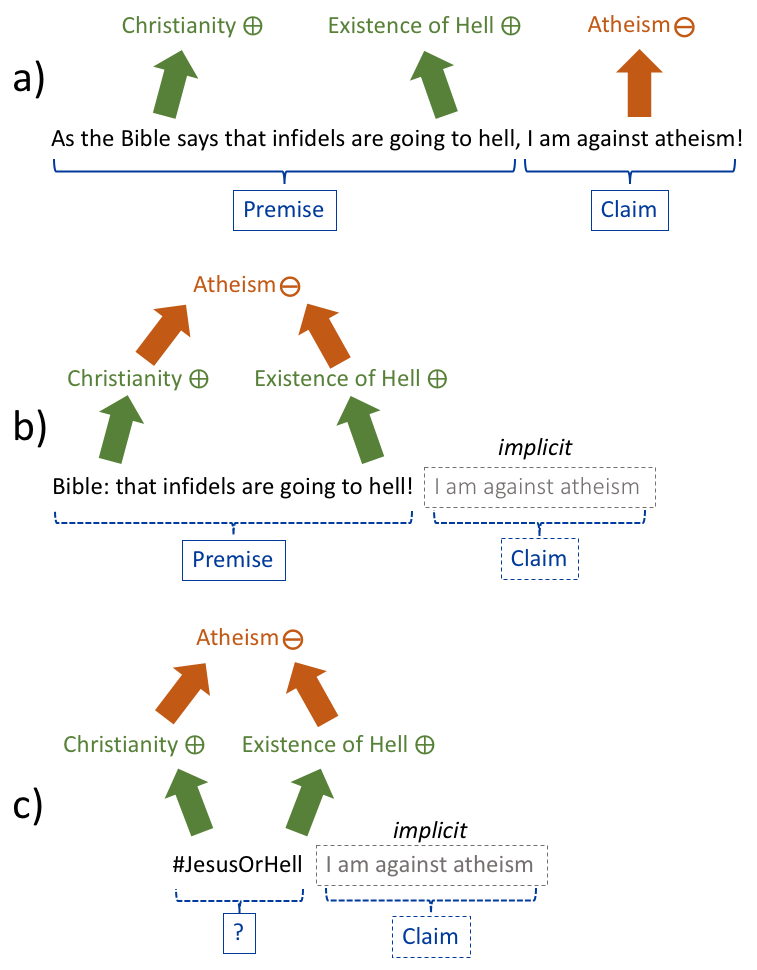
\includegraphics[width=0.49\textwidth]{figures/comparison_models_2.png}
  %}
  \caption{Stance-based vs.\ \textit{claim}-\textit{premise} model}
  \label{fig:comparison_models}
\end{figure}

In order to overcome the challenges which are described above, we introduce a new model based on a \textit{debate stance} that will in most cases be implicit, but can be inferred from one or more \textit{explicit stances} that rely on textual evidence from the utterance.
We thereby assume that an utterance is always made in the context of a certain debate.
Figure \ref{fig:comparison_models} exemplifies the assumed model and also shows it's advantages compared to a claim-premise model.
In implicit argumentation the claim usually needs to be inferred, as it is not explicitly expressed (see figure~\ref{fig:comparison_models}b).
We argue, that in the absence of explicit information, the claim always corresponds to the overall stance in the debate in which the utterance is made.

In the context of a debate about atheism, an utterance like \textit{God will judge those infidels!} expresses a stance in favor of a supernatural power (\textit{Supernatural Power}\,$\oplus$), while the actual stance on the debate target of atheism (\textit{Atheism}\,$\ominus$) is not visible but must be inferred.
Note that the debate stance might also be explicitly expressed (see figure~\ref{fig:comparison_models}a), but in implicit argumentation it has to be derived from the explicit stances.

In principle, each utterance evokes a large set of implicit stances (in a similar way as the iceberg contains a lot of invisible ice below the waterline). 
For instance, one may infer that a person uttering \textit{Bible: infidels are going to hell!} is probably in favor of praying and might have a negative stance towards issues such as abortion, same-sex marriage, etc. 
However, we argue that being in favor of Christianity already implicitly covers these stances under a common sense interpretation. 
Depending on the present informational need these targets may be more or less relevant.

Thereby, our model of implicit argumentation aligns with the \textit{Relevance Theory} proposed by \newcite{sperber1986relevance} and the \textit{Cooperative Principle} by \newcite{grice1970logic} as we also assume that utterances provide hints on the intended meaning to the recipient. Particularly, our model shares the assumption of \textit{Relevance Theory} that the precision of statements is such that a receiver can decode the meaning only by incorporating the context.

\subsection{Related Work}
In this related work section, I will briefly point to approaches and studies that serve as foundations of the proposed model and my project. 

\subsubsection{Differentiating Stance}
\label{sec:linkingStance}
In order to differentiate stance in debates, one often relies on on sub-structures, which are more explicit than the debate stance.
Controversial sub-structures in debates and their relations to stance have been studied by several researchers. 
We distinguish these works based on the origin of the sub-structures.
\newcite{swanson2015argument} and \newcite{misra2015using} extract sub-structures using text summarization techniques and then group them by a similarity measure which incorporates stance.
For instance, if two statements relate to the same target, but express different polarities they are considered to be \textit{roughly equivalent}.
Consequently, stance is modelled only indirectly but may be inferred from the grouping of statements by the similarity measure.
In addition, their approach relies on text summarization which does not make sense for very short texts such as the shown examples.
\newcite{hasan2014you} use reoccurring sub-structures on which several annotators have agreed.
\newcite{conrad2012recognizing} manually model two hierarchies of argumentative phrases with positive and negative stance as root nodes.
Each hierarchy consists of more general phrases (such as \textit{bill is politically motivated}) which are refined by phrases in the lower level of the hierarchy.
\newcite{sobhani2015argumentation} analytically define sub-debates, while \newcite{boltuzic2014back} extract them from the debating website \textit{\mbox{idebate.org}}.

\subsubsection{Stance Detection}
\label{sec:sota}
Besides having an expressive and reliable model, it is important to keep in mind that models also have to prove their practicality.
However, as approaches that fully automatize a model with both debate stance and explicit sub-structures are rare and the corresponding evaluations are highly tuned towards the used dat set and annotations.
Since there are plenty of comparable approaches for the underlying technique of automated stance detection, I will focus on describing the state-of-the-art in this area.

Most state-of-the-art approaches for stance detection are based on supervised machine learning.
Supervised learning refers to automatically inferring a classification function based on a set of training examples. 

Early approaches in stance detection adapt supervised sentiment classification techniques to distinguish between $\ominus$ and $\oplus$ stance in texts.
They rely on classifiers equipped with engineered features such as ngrams, negators, modal verbs, lexicons or dependency features \cite{walker2012stance,anand2011cats,hasan2013stance,faulkner2014automated}. 
As they do not consider the \textsc{none} class, we argue that they are not suitable for real-world applications, as these are usually confronted with noisy data and need to filter out irrelevant texts.
The consideration of the \textsc{none} class was recently established by the shared tasks on stance detection SemEval 2016 task 6 \cite{StanceSemEval2016} or the NLPCC Task 4 \cite{xu2016overview}.

While the participants in the shared tasks have used a variety of approaches, we identify two main strands.
First, knowledge-light, neural network architectures as used by the best teams in the SemEval challenge \cite{zarrella2016mitre,wei2016pkudblab}.
These approaches translate the training data in sequences of pre-trained word embeddings and feed them into neural networks.
More precisely, the top scoring approach utilizes a long-short-term-memory (LSTM) layer \cite{zarrella2016mitre}.
LSTMs are an augmentation of recurrent neural networks which utilize a special gate node (called forget gates).   
This gate node allows the LSTM layer to abstract features based on sequences with varying length.
Second, more traditional classifiers which represent the data mostly through word and character ngrams, averaged word-embeddings and sentiment features.
These representations are than used to train models with algorithms such as support vector machines (SVMs) \cite{StanceSemEval2016,xu2016overview}. 
While the results of SemEval and NLPCC show that these approaches outperform the neural approaches, neural approaches are highly competitive which underlines that it is ultimately unclear which strand is superior.

\section{Data-driven Methodology}
%\label{sec:methods}
%In this section, I will describe the methodology we follow to get evidence for the introduced model. 
%This methodology is only to bee seen as framework for the PhD project, modified according to the individual research sub-projects and -questions.

%\subsection{Data}
In order to ensure, that the made assumptions are reasonable, it is important examine the alignment to actual, real-world data.
In doing so, I attach great importance to covering a variety of different data sets to cover variability with regard to targets and domains.
By comparing methods on different data, we try to derive more general findings.

Since only a few (resp. no) data sets are available which meet our requirements, we also construct data ourselves by conducting annotation experiments.
Annotation studies typically include $>=2$ annotators who try to apply a annotation scheme (a model) to the same data.
By comparing the annotators, these studies allow valuable insights into the reliability of the annotation, which can additionally provide evidence for the validity of our model.

Annotated data also enables an examination of quantitative dependencies between the components of our model.
These patterns correspond to the interpretability of our model, as they enable to develop a deeper understanding of social media discussions.
These patterns include the frequency to which certain explicit stances occur, several explicit stances co-occur and to which explicit stances occur with a certain debate stance.

Finally, using the annotated data, we can develop and test algorithms, which is a major goal of this work.

We currently have worked with the following data sets:
\paragraph{SemEval 2016 - Task 6 \cite{mohammad2016stance}}

This data set is part of the first shared task on automated stance detection.
The organizers provided a trial, training, and test dataset of 100, 2814, and 1249 tweets, respectively for detecting stance towards five targets namely
\textit{Atheism}, \textit{Climate Change is a Real Concern}, \textit{Feminist Movement}, \textit{Hillary Clinton}, and \textit{Legalization of Abortion}.
In addition, the organizers provide an unlabelled corpus and labeled test-data towards the target \textit{Donald Trump}.

\paragraph{Atheism Stance Corpus \cite{wojatzki2016}}
In this study, we reannotate tweets on \textit{Atheism} (513 from the training set and 220 from the test set), as we found the topic to require less knowledge about specific political events from the SemEval task.
We let three annotators (two undergraduate and one graduate student of cognitive science) identify stances towards the explicit targets and the debate target.

To derive explicit targets we utilize a semi-automated, bottom-up approach that focusses on concepts that are mostly explicitly expressed by named entities and nouns.
As we want to ensure that the targets differentiate the authors' positions sufficiently, we consider the degree of association between concepts and stance polarities.
In detail, we compute the collocation coefficient $Dice$ \cite{smadja1996translating} for each word, and selected the 25 words which are most strongly associated with \textit{Atheism}\,$\ominus$ and \textit{Atheism}\,$\oplus$.
As the resulting concepts are too numerous and too fine-grained to be used in our model and ,thus, manually them into more coarse-grained targets.

\paragraph{YouTube Stance Corpus \cite{wojatzki2017youtube}}
This newly created data set contains youtube comments towards death penalty.
First, we apply a semi-automated selection to find videos that are as representative as possible and obtained a set of six videos.
Then we polled the Youtube API\footnote{\url{http://developers.google.com/youtube/}; v3-rev177-1.22.0} and received 821 comments (313 of them replies) from 614 different users with a total of 30\,828 tokens.
Using the same annotation scheme as in the SemEval task, we had three graduate students annotate each comment with stance towards death penalty and explicit stances.
As explicit targets, we rely on targets from the debating website \textit{\mbox{idebate.org}}\footnote{\url{http://idebate.org/debatabase/debates/capital-punishment/house-supports-death-penalty}} and from social media debates on \textit{\mbox{reddit.com}}.
For the reddit targets, we extracted targets from the subreddit \footnote{\url{http://www.reddit.com/r/changemyview}}, where users post controversial standpoints and invite others to challenge it.

\paragraph{Hatespeech Corpus \cite{hatespeech2016}}
As I argue that one can consider hate speech as an extreme, unpleasant form of stance taking, I also report on the resources that were created in the interdisciplinary working group \textit{hate speech}.
In the IWG we have so far conducted two studies and corresponding data sets.
In the first study \cite{hatespeech2016}, we created a german hate speech corpus and conducted an experiment in which we demonstrate that hate speech is a (too) fuzzy concept and that is very hard to reach consensus on whether a tweet is hate speech or not.
In the second study \cite{hatespeech2017implicitness}, we shed light on the influence of implicitness on hate speech annotations and show an measurable influence which is however, moderated by e.g. content variables. 

\paragraph{IberEval - Stance and Gender detection in tweets on Catalan Independence \cite{iberEval2017}}
This data set is part of a shared task on automated stance detection in tweets on Catalan Independence.
So far the organisers have released only the train set, containing 4319 tweets in Spanish and 4319 in Catalan.
All the tweets were labeled with the SemEval scheme.
%
%
%\subsection{Patterns}
%The section dimension of our methodology framework deals with quantitative dependencies between the components of our model.
%These patterns correspond to the itnterpretability of our model, as they enable to develop a deeper understanding of social media discussions.
%These patterns include the frequency to which certain explicit stances occur, several explicit stances co-occur and to which explicit stances occur with a certain debate stance. 
%
%\subsection{Machine Learning}
%Since a major goal on my PhD project is to develop new algorithms for analyzing discussions, it is necessary to shortly outline necessary details of used paradigms and implementation.
%As mentioned above, machine learning approaches are the dominant technique in stance detection (or natural language processing).
%This dominance is reasonable, as especially comes in large amounts and high variability which cannot be handled without such methods.
%
%Machine learning needs a representation of the data.
%Recently, there has been a shift in NLP from providing this representation through engineered features to automatically extract features from raw data. 
%
%
%CV
%preprocessing
%word embedings
%DKPRO-TC
%keras.io


\section{Published Results}
\subsection{ltl.uni-due@SemEval Task 6 \cite{wojatzki2016stance}}
We participated in the \textit{\mbox{SemEval} 2016 Task 6: Detecting Stance in Tweets} which represents the first shared task on stance detection that tried to explore the state-of-the-art.

Figure \ref{fig:sketch1} gives a overview on our system for automated stance detection (for a a more detailed explanation see \newcite{wojatzki2016stance}).

\begin{figure*}
  \centering
  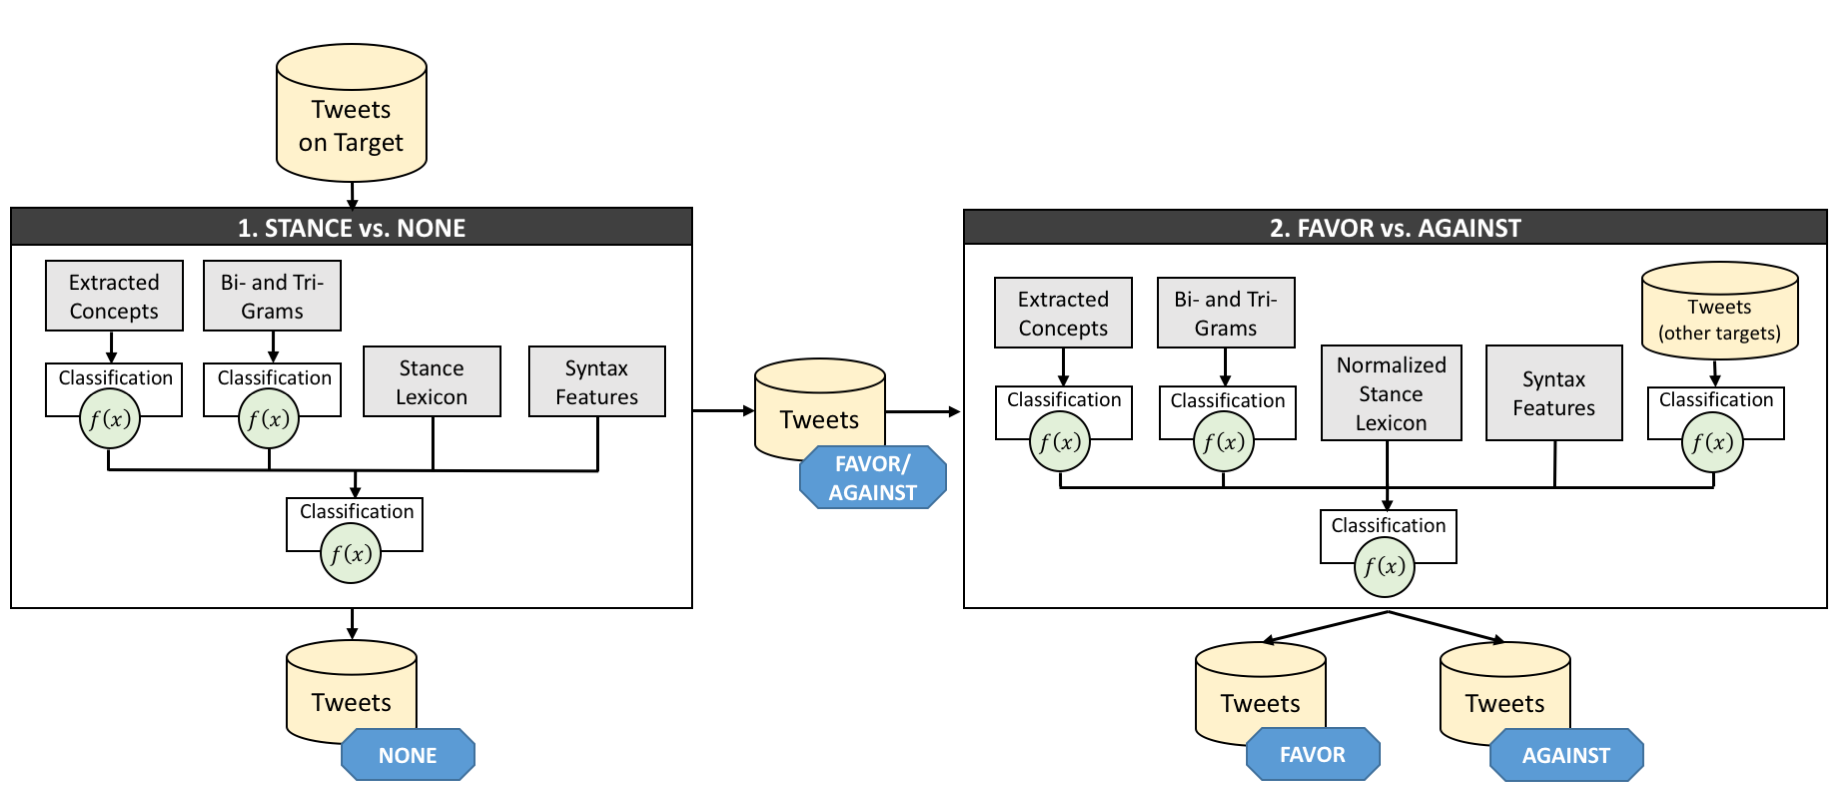
\includegraphics[scale=0.25]{figures/stance_skizze_new.png}
  \caption{Overview on the sequence of stacked classifications that is used for the supervised setting (subtask A)}
  \label{fig:sketch1}
\end{figure*}


As the targets are quite different, we train a separate classifier for each of them. 
Additionally, we split the three-way classification into a stacked classification, in which we first classify whether the tweet contains any stance (classes $\oplus$ and $\ominus$) or no stance at all (class \textsc{None}).
In a second step, we classify the tweets labeled as containing a stance as $\oplus$ or $\ominus$.
Our analysis revealed that simple word features are best suited to learn the relationship between tweets and stance.

As demonstrated by the task organizers none of them beats the provided baseline which is  a support vector machine equipped with character and word ngrams \cite{StanceSemEval2016}.


\paragraph{Lessons Learnt}
In general, the results suggest that the performance of the state-of-the-art is significantly better than a random or a majority class baseline, but still leaves huge room for improvements. 
The state-of-the-art mainly uses lexical/lexical semantic knowledge such as ngrams and wordembeddings.
In a post-hoc analysis they show that this baseline profits from leveraging target specific unlabelled data \cite{mohammad2016stance}.


\subsection{Stance-based Argument Mining \cite{wojatzki2016}}
In this publications we postulated the model which is explained in section \ref{fig:SBAM}.
As explained in the previous section, we applied this model to a sub set of the SemEval data.
Figure \ref{fig:kappa_subTargets} shows the Fleiss' $\kappa$ for the annotation.
\begin{figure*}[ht!]
\centering
\begin{tikzpicture}
        \begin{axis}[
        xbar,
            symbolic y coords={No Evidence,  Life After Death, Same-Sex Marriage, Religious Freedom, USA, Conservatism, Freethinking,no explicit target, Supernatural Power, Secularism, Islam, Christianity, , Atheism},
            ytick=data, 
            bar width= 5,
            width=.8\textwidth,
           % yticklabel style={rotate=45, anchor=east, align=center},
            height=.4\textwidth,
            xmin = 0, 
			xmax = 1,
			nodes near coords,
			every node near coord/.append style={font=\small,black},
			enlarge y limits=0.04,
			xlabel=Fleiss' $\kappa$,
			yticklabel=\ifthenelse{\equal{\tick}{no explicit target}}{\textit{no explicit target}}{\tick}]
          ]
            \addplot[xbar,orange,fill=orange!25] coordinates {
            	(0.72,Atheism)
                (0.85,Christianity)
                (0.81,Islam)
                (0.76,Secularism)
				(0.73,Supernatural Power)
                (0.73,Freethinking)
                (0.73,no explicit target)
				(0.63,Conservatism)
                (0.57,USA)
                (0.52,Religious Freedom)
				(0.51,Same-Sex Marriage)
				(0.43,Life After Death)
				(0.31,No Evidence)
            };
        \end{axis}
       % \draw [ultra thick, dashed, draw=gray](2.2,4.8)--(2.2,0); %separator (is not positioned very clever at the moment)
    \end{tikzpicture}
    \caption{Inter-annotator agreement of the debate stance \textit{Atheism} and explicit stances}
\label{fig:kappa_subTargets}
   \end{figure*}
  
As shown in figure~\ref{fig:kappa_subTargets}, we obtain a Fleiss' $\kappa$ of 0.72 for the annotation of the debate stance which is comparable to scores in the literature. 
Two explicit targets (\textit{Christianity} and \textit{Islam}) yield especially high agreement, because they are associated with clear signal words such as \textit{Jesus} and \textit{Quran}.
Other targets such as \textit{Secularism} are rather abstract.
They hardly involve special signal words but still gain high agreements, which shows that our annotators did not just recognize certain keywords, but also reliably annotate more abstract targets.
An error analysis for the target \textit{Same-Sex Marriage} shows that there is disagreement if the tweet contains a stance towards gay rights in general but not to gay marriage.
Finally, we obtain a $\kappa$ of 0.63 for the joint decision on both the debate and the explicit targets.

\begin{figure}[ht!]
\centering
  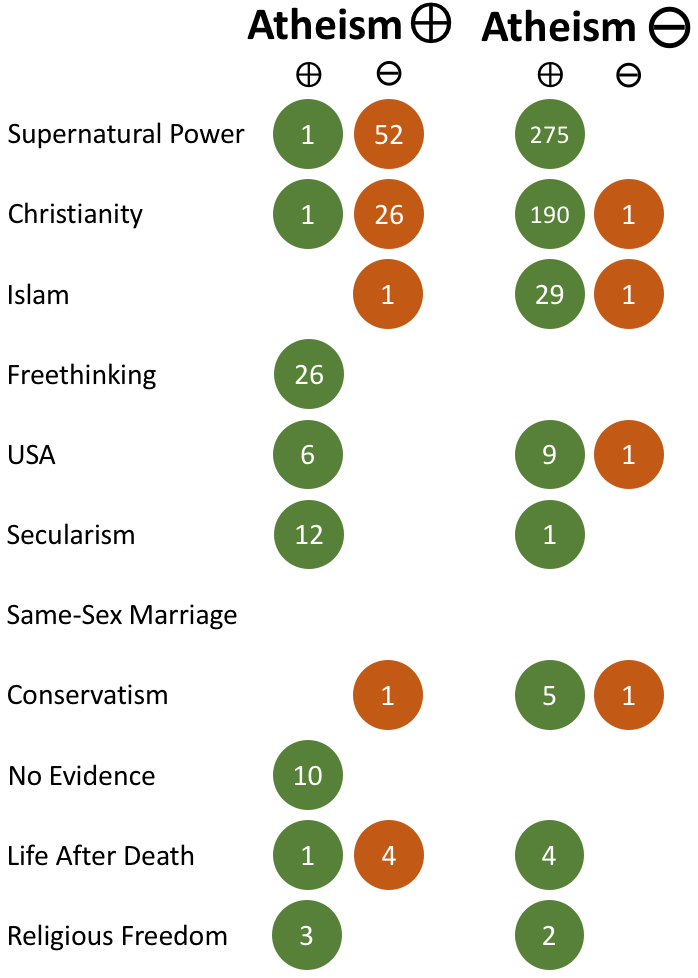
\includegraphics[width=0.45\textwidth]{figures/patterns_flat.png}
  \caption{Frequency of explicit stances grouped according to debate stance}
  \label{fig:patterns_flat}
\end{figure}

\paragraph{Patterns}
In order to inspect usage patterns of explicit stance taking, we must agree on one annotation for each tweet.
Since we do not assume that there are differences in the quality of the three annotators, we rely on a majority vote to compile a final annotation. 

Figure~\ref{fig:patterns_flat} visualizes the frequency of the explicitly taken stances for Atheism\,$\oplus$ and Atheism\,$\ominus$.
It shows that there are significant differences in the argumentation patterns between the two camps.
As expected, if advocates of atheism are against a target such as \textit{Christianity}, the opponents are mostly in favor of it or do not mention it.

From these analysis we can conclude that stable patterns of argumentation using explicit stances other than the debate stance exist.
This is a strong indication for the validity of our assumption that the debate stance can be inferred from explicitly expressed stances.

\paragraph{Machine Learning}

In order to investigate how well our model can be assigned automatically, we conduct classification experiments and compare with suitable baselines.

We re-implement a state-of-the-art classifier, run experiments in the manner of a ten-fold cross-validation and report micro averaged $F_1$.
Compared to the majority class baseline ($F_1=.49$), we obtain a higher $F_1$ of $.66$ for the debate stance classification..
In order to evaluate the usefulness of explicit stances for inferring the debate stance, we use the predictions of explicit targets as features for stance classification.
This stacked classifier performs en par ($.65$) with the n-gram based classifier.

To estimate the potential of explicit stance features for classifying the debate stance, we add an oracle condition to our experiments in which we assume that the classification of explicit stances is done correctly.
This classifier using only the manually annotated explicit stances yields an $F_1$ score of $.88$ showing that large improvements over the state of the art are possible if explicit stances can be more reliably classified.

\paragraph{Lessons Learnt}
The proposed model can be reliably annotated and provides interesting quantitative insights in discussions. 
Stacking classification of explicit targets is currently not improving debate stance classifications, but performs en par. 

\section{Unpublished Results/ Under Review}

\subsection{Neural and Non-neural Stance Classifiers learn Sub-debates \cite{wojatzki2017youtube} }

As a result of the previous conducted experiments, we hypothesize that stance classifiers internally learn structures that correspond to explicit stances. 
Thus, we conducted suitable experiments on the YouTube Stance Corpus \cite{wojatzki2017youtube}.

For reasons of comparability, we compute \textit{Fleiss'} $\kappa$  between the three annotators to assess reliability.
These scores are shown in Figure \ref{fig:kappa_cmvTargets}.
For the debate stance, we obtain a value of .66 which is in a similar to the previous experiments.
Overall, we obtain a mixed picture for the annotation of explicit stances, as we get $\kappa$ values in a range from .13 up to .87. 
While the majority of sub-debates is annotated with a $\kappa$ of above .6, there are significant deviations downwards such as \textit{Financial Burden} with a $\kappa$ of .26.

\begin{figure*}[ht!]
\centering
\resizebox{\textwidth}{!}{%
\begin{tikzpicture}
        \begin{axis}[
        xbar,
            symbolic y coords={Certainty Unachievable,Replace Life-Long, Abortion,Strangulation,Heinous Crimes,Use Bodies,More Quickly,More Harsh,Gunshot,Electric Chair, ,Financial Burden, Miscarriages, Eye for an Eye,State Killing, Preventive,Irreversible,Deterring,Closure, Overcrowding, ,Explicit Debate Stance, ,Debate Stance},
            ytick=data, 
            bar width= 5,
            width=.8\textwidth,
           % yticklabel style={rotate=45, anchor=east, align=center},
            height=.52\textwidth,
            xmin = 0, 
			xmax = 1,
			nodes near coords,
			every node near coord/.append style={font=\small,black},
			enlarge y limits=0.04,
			tick label style={font=\small},
			tick label style={font=\small},
			xlabel=Fleiss' $\kappa$,]
          ]
           \addplot[xbar,orange,fill=orange!25] coordinates {
            (0.66,Debate Stance)
             (0.64,Explicit Debate Stance)
             (0.87,Electric Chair)
             (0.74,Gunshot)
             (0.23,Replace Life-Long)
             (0.56,Use Bodies)
       		 (0.42,Heinous Crimes)
	         (0.3,Abortion)
             (0.13,Certainty Unachievable)
             (0.71,More Harsh)
			 (0.7,More Quickly)
		     (0.4,Strangulation)
		     (0.71,Deterring)
             (0.40,Eye for an Eye)
             (0.77,Overcrowding)
             (0.64,Preventive)
             (0.6,State Killing)
			 (0.29,Miscarriages)
             (0.7,Irreversible)
             (0.72,Closure)
             (0.26,Financial Burden)

            };
        \end{axis}
        \draw [decorate, decoration={brace,amplitude=8pt,raise=1pt,mirror}] (10.5,3.1) -- (10.5,5.5) 
            		node[rotate=270,font=\small, midway, yshift=5mm]{Idebate-Set};
        \draw [decorate, decoration={brace,amplitude=8pt,raise=1pt,mirror}] (10.5,0.15) -- (10.5,2.8) 
            		node[rotate=270,font=\small, midway, yshift=5mm]{Reddit-Set};
       % \draw [ultra thick, dashed, draw=gray](2.2,4.8)--(2.2,0); %separator (is not positioned very clever at the moment)
    \end{tikzpicture}
    }
    \caption{Inter-annotator agreement for the debate stance, explicitly expressed debate stance, the Idebate Set and the Reddit Set.}
\label{fig:kappa_cmvTargets}
   \end{figure*}

\paragraph{Patterns}
As in the Atheism corpus, we again inspect quantitative patterns.
These dependencies are visualized in Figure \ref{table:occurrenceAndCoOccurrence}.
Slightly over 50\% of comments do not have any explicit target, but this is mainly due to the \textsc{None} cases that do not express any stance at all.
For the polar instances ($\ominus$ + $\oplus$), 389 out of 496 comments (78\%) have one or more explicit target.


\begin{table*}[]
\centering
\footnotesize
\resizebox{\textwidth}{!}{
\begin{tabular}{r|c||c|cccccccccc|ccccccccc}
%\toprule
 \textbf{Sub-Debate} & & \tnumb{1} &\tnumb{2} & \tnumb{3}&\tnumb{4} & \tnumb{5}& \tnumb{6}& \tnumb{7} & \tnumb{8}  & \tnumb{9}& \tnumb{10}& \tnumb{11}  & \tnumb{12} & \tnumb{13} & \tnumb{14} & \tnumb{15} & \tnumb{16}  & \tnumb{17} & \tnumb{18} & \tnumb{19}& \tnumb{20} \\ 
\midrule
Explicit Debate Stance   &    \tnumb{1}   &    {\ul \textbf{87}}   & 1 & 8 & 13 & 3 & 0 & 4 & 0 & 5 & 9 & 0 & 9 & 1 & 1 &    \cellcolor[HTML]{FFCE93}15   & 1 & 1 & 2 & 1 &  0 \\
\hline
Closure   &    \tnumb{2}   & 1 &    {\ul\textbf{19}}   &    \cellcolor[HTML]{FFCE93}3   &    \cellcolor[HTML]{F8A102}7   & 2 & 1 & 1 & 0 &    \cellcolor[HTML]{FFCE93}3   & 1 & 0 & 1 & 0 & 1 &    \cellcolor[HTML]{F8A102}6   & 2 & 0 & 1 & 1 &  0 \\
Deterring   &    \tnumb{3}   & 8 & 3 &    {\ul\textbf{55}}   & 5 & 6 & 1 & 2 & 1 & 6 & 3 & 0 & 4 & 0 & 1 & 6 & 2 & 3 & 3 & 0 &  0 \\
Eye for an Eye   &    \tnumb{4}   & 13 & 7 & 5 &    {\ul\textbf{87}}   & 2 & 1 & 0 & 1 & 6 & 9 & 2 & 5 & 2 & 3 &    \cellcolor[HTML]{F8A102} 45   & 2 & 5 & 6 & 3 &  0 \\
Financial Burden   &    \tnumb{5}   & 3 & 2 & 6 & 2 &    {\ul\textbf{46}}   & 2 & 2 & 2 & 2 & 0 & 0 &    \cellcolor[HTML]{FFCE93}7   & 0 & 5 & 6 & 1 &    \cellcolor[HTML]{FFCE93}11   & 4 & 1 &  0 \\
Irreversible   &    \tnumb{6}   & 0 & 1 & 1 & 1 &    \cellcolor[HTML]{FFCE93}2   &    {\ul\textbf{11}}   & 1 & 0 & 0 &    \cellcolor[HTML]{FFCE93}2   & 0 & 1 & 0 & 0 & 0 & 0 & 0 &    \cellcolor[HTML]{FFCE93} 2   & 0 &  0 \\
Miscarriages   &    \tnumb{7}   &    \cellcolor[HTML]{FFCE93}4   & 1 & 2 & 0 & 2 & 1 &    {\ul\textbf{19}}   & 0 & 0 & 1 & 0 &    \cellcolor[HTML]{F8A102}6   & 0 & 0 & 1 & 0 & 0 & 0 & 0 &  0 \\
Overcrowding   &    \tnumb{8}   & 0 & 0 &    \cellcolor[HTML]{FFCE93}1   &    \cellcolor[HTML]{FFCE93}1   &    \cellcolor[HTML]{F8A102}2   & 0 & 0 &    {\ul\textbf{6}}   & 0 & 0 & 0 &    \cellcolor[HTML]{FFCE93}1   & 0 &    \cellcolor[HTML]{FFCE93}1   &    \cellcolor[HTML]{F8A102}3   & 0 & 0 & 0 & 0 &  0 \\
Preventive   &    \tnumb{9}   &    \cellcolor[HTML]{FFCE93}5   & 3 &    \cellcolor[HTML]{FFCE93}6   &    \cellcolor[HTML]{FFCE93}6   & 2 & 0 & 0 & 0 &    {\ul\textbf{27}}   & 2 & 1 & 2 & 0 & 2 &    \cellcolor[HTML]{FFCE93}8   & 2 & 2 & 1 & 2 &  0 \\
State Killing   &    \tnumb{10}   &    \cellcolor[HTML]{FFCE93}9   & 1 & 3 & 9 & 0 & 2 & 1 & 0 & 2 &    {\ul\textbf{38}}   & 0 & 5 & 0 & 1 &    \cellcolor[HTML]{FFCE93}8   & 0 & 0 & 3 & 1 &  0 \\
\midrule
Abortion   &    \tnumb{11}   & 0 & 0 & 0 &    \cellcolor[HTML]{FFCE93}2   & 0 & 0 & 0 & 0 & 1 & 0 &    {\ul\textbf{7}}   & 0 & 0 & 0 &    \cellcolor[HTML]{FFCE93}3   & 0 & 1 & 1 & 1 &  0 \\
Certainty Unachievable   &    \tnumb{12}   &    \cellcolor[HTML]{FFCE93}9   & 1 & 4 & 5 & 7 & 1 & 6 & 1 & 2 & 5 & 0 &    {\ul\textbf{57}}   & 0 & 2 & 8 & 0 & 7 & 4 & 1 &  0 \\
Electric Chair   &    \tnumb{13}   &    \cellcolor[HTML]{FFCE93}1   & 0 & 0 &    \cellcolor[HTML]{F8A102}2   & 0 & 0 & 0 & 0 & 0 & 0 & 0 & 0 &    {\ul\textbf{6}}   &    \cellcolor[HTML]{FFCE93}1   &    \cellcolor[HTML]{F8A102}3   &    \cellcolor[HTML]{FFCE93}1   & 0 &    \cellcolor[HTML]{F8A102}2   & 0 &  0 \\
Gunshot   &    \tnumb{14}   & 1 & 1 & 1 & 3 &    \cellcolor[HTML]{FFCE93}5   & 0 & 0 & 1 & 2 & 1 & 0 & 2 & 1 &    {\ul\textbf{22}}   &    \cellcolor[HTML]{FFCE93}4   & 1 &    \cellcolor[HTML]{F8A102}8   & 0 &    \cellcolor[HTML]{FFCE93}4   &  1 \\
Heinous Crimes   &    \tnumb{15}   &    \cellcolor[HTML]{FFCE93}15   & 6 & 6 &    \cellcolor[HTML]{F8A102} 45   & 6 & 0 & 1 & 3 & 8 & 8 & 3 & 8 & 3 & 4 &    {\ul\textbf{96}}   & 7 & 5 & 7 & 5 &  0 \\
More Harsh   &    \tnumb{16}   & 1 & 2 & 2 & 2 & 1 & 0 & 0 & 0 & 2 & 0 & 0 & 0 & 1 & 1 &    \cellcolor[HTML]{FFCE93}7   &    {\ul\textbf{20}}   & 0 & 1 & 1 &  1 \\
More Quickly   &    \tnumb{17}   & 1 & 0 & 3 &    \cellcolor[HTML]{FFCE93}5   &    \cellcolor[HTML]{F8A102}11   & 0 & 0 & 0 & 2 & 0 & 1 &    \cellcolor[HTML]{FFCE93}7   & 0 &    \cellcolor[HTML]{FFCE93}8   &    \cellcolor[HTML]{FFCE93}5   & 0 &    {\ul\textbf{30}}   & 0 & 2 &  0 \\
Replace Life-Long   &    \tnumb{18}   & 2 & 1 & 3 &    \cellcolor[HTML]{FFCE93}6   & 4 & 2 & 0 & 0 & 1 & 3 & 1 & 4 & 2 & 0 &    \cellcolor[HTML]{FFCE93}7   & 1 & 0 &    {\ul\textbf{35}}   & 0 &  0  \\
Strangulation   &    \tnumb{19}   & 1 & 1 & 0 &    \cellcolor[HTML]{FFCE93}3   & 1 & 0 & 0 & 0 &    \cellcolor[HTML]{FFCE93}2   & 1 & 1 & 1 & 0 &    \cellcolor[HTML]{F8A102}4   &    \cellcolor[HTML]{F8A102}5   & 1 &    \cellcolor[HTML]{FFCE93}2   & 0 &    {\ul\textbf{12}}   &  1 \\
Use Bodies   &    \tnumb{20}   & 0 & 0 & 0 & 0 & 0 & 0 & 0 & 0 & 0 & 0 & 0 & 0 & 0 & 1 & 0 & 1 & 0 & 0 & 1 &    {\ul\textbf{8}} \\
\bottomrule
\end{tabular}
}
\vspace*{-4.5mm}
\caption{Frequency of sub-debates (bold-faced, underlined cells on main diagonal) and their co-occurrences with other sub-debates. We highlight cases (row-wise) in which a sub-debate frequently co-occurs with another. Light orange for more than 15\% overlap, and dark orange for more than 30\%.}
\vspace*{-3mm}
\label{table:occurrenceAndCoOccurrence}
\end{table*}

In the main diagonal of the table, we visualize how often a certain explicit target occurrs in the data.
Overall, none of the two inventories can be clearly preferred over the other, as both contain frequent and thus useful sub-debates and ones that occur infrequently or not at all.

We observe, that the most frequent targets(\textit{Heinous Crimes} and \textit{Eye for an Eye}) are often used as proxies for a general position in the debate, such as in the comment \textit{If someone raped and killed your family, do you think they should continue to exist?}.
The second most common group are more specific sub-debates (e.g.\ \textit{Deterring}) which occur in about $10\%$ of the polar instances.
The other sub-debates seem to cover rather marginal positions in the debate. 

W.r.t.\ cooccurrences, we observe that targets are rarely combined, as only \textit{eye for an eye} co-occurs in over 50\% of its appearances with others.
The two most frequent targets relatively co-occur most with other targets (see column 5 and 15 in Table~\ref{table:occurrenceAndCoOccurrence}), which underlines their role as proxies for a general position. 
As both sub-debates contain the demand of the death penalty for certain crimes, unsurprisingly, they also co-occur quite frequent.

While most targets are rarely backed up with others, e.g.\ \textit{Gunshot}, \textit{Strangulation} or \textit{Electric Chair} are combined frequently (rows 13,14 and 19). 
We argue that they tend to be rather complementary´and used to support other targets or form logical units with them.
For instance, \textit{Gunshot} frequently co-occurs with \textit{More Quickly}, which is reasonable if one considers that an execution could be performed very quickly by shooting.

\paragraph{Machine Learning}
To get insights in the learned structure, we examine how well classifiers perform on comments that contain a certain explicit target. 
Therefore, we calculate the performance on subsets of the data, which correspond to the instances annotated with the respective target.

Ee implement prototypical representatives of the two main strands of approaches -- an SVM and a neural architecture with a (Bi)LSTM layer in its core. 
We calculate the classification performance using leave-one-out cross-validation on the video level and the micro-average of $F_1\oplus$ and $F_1\ominus$ for comparability.
Figure~\ref{fig:performance_perSubtargets} visualizes the corresponding results.

Overall, we achieve an $F_1$-score of $.45$ for both classifiers.
If we consider only the comments that contain a sub-debate, classification works considerably better ($.53$ for LSTM and SVM).
However, if we exclude comments with sub-debates, we observe a large drop in classification performance (LSTM: $.24$, SVM: $.23$).

Overall, we do not observe major differences between the two sub-debate inventories regarding classification performance.

\begin{figure*}[ht!]
\centering
%\resizebox{\textwidth}{!}{%
\begin{tikzpicture}
        \begin{axis}[
        xbar,
            symbolic y coords={Use Bodies, Strangulation, Replace Life-Long, More Quickly,More Harsh,Heinous Crimes,Gunshot, Electric Chair,Certainty Unachievable, Abortion, , State Killing, Preventive,Overcrowding, Miscarriages,Irreversible, Financial Burden,Eye for an Eye,Deterring,Closure, , Explicit Debate Stance, ,All Sub-debates Excluded,All Sub-debates,All},
            ytick=data, 
            bar width= 3,
            width=.7\textwidth,
           % yticklabel style={rotate=45, anchor=east, align=center},
            height=.65\textwidth,
            xmin = 0, 
			xmax = 1,
			nodes near coords,
			every node near coord/.append style={font=\scriptsize,black},
			enlarge y limits=0.02,
			tick label style={font=\small},
			tick label style={font=\small},
			xlabel=micro-average of $F_1\oplus$ and $F_1\ominus$,]
          ]
            \addplot[xbar,blue,fill=blue!35] coordinates {
              (0.45,All)
              (0.23,All Sub-debates Excluded)
              (0.53,All Sub-debates) 
              (0.55,Explicit Debate Stance)
              (0.50,Deterring)
              (0.66,Electric Chair)
           	  (0.36,Use Bodies)
           	  (0.32,Strangulation)
           	  (0.55,Overcrowding)
              (0.58,Eye for an Eye)
              (0.54,Preventive)
              (0.60,State Killing)
			  (0.61,Miscarriages)
              (0.74,Irreversible)
              (0.81,Closure)
              (0.65,Financial Burden)
              (0.47,Gunshot)
              (0.55,Replace Life-Long)
       		  (0.59,Heinous Crimes)
	          (0.66,Abortion)
              (0.56,Certainty Unachievable)
              (0.64,More Quickly)
              (0.63,More Harsh)
			  };
			   \addplot[xbar,red,fill=red!35] coordinates {
              (0.45,All)
              (0.24,All Sub-debates Excluded)
              (0.53,All Sub-debates) 
              (0.52,Explicit Debate Stance)
              (0.37,Deterring)
              (0.66,Electric Chair)
           	  (0.77,Use Bodies)
           	  (0.70,Strangulation)
           	  (0.83,Overcrowding)
              (0.60,Eye for an Eye)
              (0.66,Preventive)
              (0.45,State Killing)
			  (0.34,Miscarriages)
              (0.38,Irreversible)
              (0.65,Closure)
              (0.62,Financial Burden)
              (0.54,Gunshot)
              (0.53,Replace Life-Long)
       		  (0.77,Heinous Crimes)
	          (0.66,Abortion)
              (0.43,Certainty Unachievable)
              (0.57,More Quickly)
              (0.6,More Harsh)
			  };
			   \draw [decorate, decoration={brace,amplitude=15pt,raise=1pt,mirror}] (90,105) -- (90,200) 
            		node[rotate=270,font=\small, midway, yshift=8mm]{Idebate-Set};
            	\draw [decorate, decoration={brace,amplitude=15pt,raise=1pt,mirror}] (90,2) -- (90,95) 
            		node[rotate=270,font=\small, midway, yshift=8mm]{Reddit-Set};
			  \legend{SVM, LSTM}
        \end{axis}
        \draw [thin, densely dashed, draw=darkgray](4.328,8.8)--(4.328,0); %separator (is not positioned very clever at the moment)
    \end{tikzpicture}
%    }
	\vspace*{-4mm}
    \caption{Stance classification performance by sub-debate}
    \vspace*{-3mm}
\label{fig:performance_perSubtargets}
   \end{figure*}

Interestingly, some of the sub-debates that cause problems for the LSTM achieve relatively high scores using the SVM. 
For example, the performance on instances annotated with \textit{Overcrowding} is .38 for the LSTM, but .74 for the SVM.
However, we also see targets, in which the situation is inverted, e.g.\ for \textit{Use Bodies} we obtain a much higher value (.77) for the LSTM than for the SVM (.36).

To better understand the interesting differences between the neural and non-neural approach, we examine how strongly they rely on the textual markers of the targets.
For that reason, analogous to an ablation test, we conduct experiments in which we remove the textual markers and examine the impact on the classification performance.
As these markers indicate the explicit stance and thus should be especially important for learning models, we expect a decline in performance.
Overall, the average drop of the LSTM is significantly bigger than that of the SVM, which means that the LSTM's representation is more dependent on the markers than the SVM.
Since the LSTM's loss is -- especially in the frequent targets -- notable, we assume that the internal LSTM representation is semantically closer to the annotated explicit stances.
Contrary, the SVM representation is more robust against removed textual evidence from which we infer that its model is more shallow.
   
\paragraph{Lessons Learnt}
Indeed, we could gather evidence for our assumption that stance classifiers internally learn structures that correspond to explicit stances.
In addition, we show the different algorithms strongly differ in which targets they capture and with respect to robustness.

\subsection{Neural and Non-neural Stance Detection in Tweets on Catalan Independence \cite{wojatzki2017ibereval}}

In this work, we try to utilize the findings described to improve stance detection.
As shown above, neural and non-neural approaches make different errors and also have different strengths.
Consequently, we hypothesize that one should be able combine the strengths of both models into a superior, hybrid system.
We validate this hypothesis by participating in the first shared task on stance detection in tweets on catalan independence \cite{iberEval2017}.
I here want to outline that I don't speak these languages and that we did not make use of any language-specific models or tools.

In our approach, we first implement prototypical representatives of the two strands, namely and a neural architecture with a (Bi)LSTM layer in its core and an SVM.
Subsequently, we built a third system that automatically decides whether a tweet should be classified with the neural or the non-neural system. 
Therefore, we first labeled every tweet with whether the SVM's respectively the LSTM's prediction was wrong or false. 
We than train an decision tree (weka's J48) for each approach to automate this decision. 
The trees are equipped with word n-gram coverage, embedding coverage, type token ratio and length features which are suspected of having an influence on the classifiability through the systems. 
Unfortunately, the performance of this classification still needs heavy improvement in future work. 
Based on these classifications we conduct a final decision. 
In case the system could not derive preference towards one system as both systems are recommend or none, we rely on the SVM as its performance is overall better.

Table \ref{table:Performance_iberstance_train} gives an overview on the performance (micro F) on the training data.
\begin{table}[]
\centering
\begin{tabular}{lll}
                                          & \textbf{Catalan} & \textbf{Spanish} \\
                                          \toprule
\textbf{SVM}                              &    0.80              &    0.70              \\
{\color[HTML]{656565} - embeddings}       &     0.79             &    0.70             \\
{\color[HTML]{656565} - character ngrams} &     0.78             &    0.70              \\
{\color[HTML]{656565} - word ngrams}      &     0.78             &    0.68             \\
\textbf{(Bi-)LSTM}                        &     0.75             &     0.66             \\
\textbf{Hybrid}                         &     0.80             &     0.70          \\
\bottomrule      
\end{tabular}
\caption{Micro averaged F$_1$-score obtained from the 10-fold crossvalidation. For the SVM we show the results of an feature ablation test.}
\label{table:Performance_iberstance_train}
\end{table}

Until now, there are only preliminary results of the performance on the test data.
Nevertheless Table \ref{table:Performance_iberstance_test} gives an overview on the performance on the training data, as reported by the organizers.
Note, that the results are reported in terms of the macro-average of $F_1\oplus$ and $F_1\ominus$.


Table \ref{table:Performance_iberstance_test} gives an overview on the performance (micro F) on the training data.
\begin{table}[]
\centering
\begin{tabular}{lll}
                                          & \textbf{Catalan} & \textbf{Spanish} \\
                                          \toprule
\textbf{SVM}                              &    0.43             &    0.42              \\
\textbf{(Bi-)LSTM}                        &     0.28             &     0.37             \\
\textbf{Hybrid}                         &     0.44             &       0.43        \\
\bottomrule      
\end{tabular}
\caption{Macro-average of $F_1\oplus$ and $F_1\ominus$ obtained from the train-test split, as reported by the organizers.}
\label{table:Performance_iberstance_test}
\end{table}

For both languages we are ranked 5th out of 12 participating teams.
For both the languages and splits, we hardly see a difference between the hybrid and the SVM system. 
This is probably due to the used heuristic, which uses the SVM prediction in cases were we cannot be sure about a decision.
However, as the the hybrid and the svm prediction is still significantly different, we still see a high potential of hybrid approaches.
As described, future work should focus on a more accurate type prediction or more advanced heuristics.

\paragraph{Lessons Learnt}
We could not demonstrate a clear superiority of a hybrid approach.
However, the obtained results outline its potential and promising directions of further improvements.

\section{Ongoing Activities}

\subsection{Interactive Stance}
In the experiments shown so far, we faced two recurrent problems: a) Creating data with high quality is time consuming and difficult  and b) without the incorporation of additional data, state-of-the-art approaches reach performance limits which are far from perfect. 
The internet and especially social media is full of discussions which could serve as such additional data, however, these discussions do not have the structure that is needed by the algorithms.
In order, to overcome these problems we propose an interactive process with which one can rapidly create training data and classifiers.
At its core the process grants the user access to thousands of online debates in an aggregated form.
Users can arrange these aggregates based on whether they think the corresponding debate is in favor or against a given target.

The prototype is currently under development.
So far we have crawled 2 of the 7 appropriate debate websites and already collected 57\,316 debates containing 339\,472 utterances.
We already offer access via a newly developed webinterface.  
A fast access to the aggregates is currently implemented via an apache solr index.
For linguistic preprocessing such as tokenization, we rely on dkpro.

We plan to evaluate the effectiveness and efficiency of the approach on the previously described data sets in English.
As users should be able to iteratively refine their arrangement, we already add a feedback mechanism that evaluates the resulting model.
As this evaluation is time critical, we cannot apply (computational) costly machine-learning algorithms.
Consequently, we rely on a heuristic scoring function.
To this end, we create stance lexicons by calculating the \textit{dice} distribution on the selected favor and against texts.
Subsequently, we define an upper and lower threshold on the resulting distribution.
The upper threshold indicates that the values above are considered as $\oplus$.
Accordingly, the lower threshold indicates that values below are considered as $\ominus$.
Thus, all other values correspond to the \textsc{none} class.
We than calculate a mean polarity for each of the texts which are to be evaluated and assign a label based on the thresholds.

In order to support the selection and arrangement of aggregates, we plan to add a support mechanism that shows the lexical overlap between selected aggregates and the data which is to be classified. 
Currently, we are working on two major problems: a) speed of analysis and data access and b) better heuristics for finding thresholds. 

After completing and deploying the prototype, we will conduct a user study in which we control for several parameters and variants of the process such as threshold for the heuristic classification and support mechanisms.


\subsection{Target Specific Embeddings}
As shown by the post-hoc analysis of the SemEval task, it is beneficial to incorporate the semantics of a domain by using domain specific word-embeddings.
Similarly, in sentiment analysis, studies demonstrate the possibility to boost performance by learning sentiment and topic specific word embeddings from heuristically labeled data \cite{ren2016improving,lan2016three,tang2016sentiment}.
The following example illustrates the assumed mechanism:
In the common sense, the words \textit{email} and \textit{scandal} are not related.
However, in the context of \textit{Hillary Clinton} both words are connected by a strong relationship.

In order to systematically examine this intuition, we constructed a set of words that should be subject to such a semantic shift in the 5 SemEval targets.
Therefore, we semi-automatically selected 20 words per target by using statistical association with the polarity classes (dice) and manual inspection and pairing.
As control items we added 20 items from the \cite{finkelstein2001placing} (which is traditionally used in studies on semantic similarity/relatedness).

The study is currently still running.
So far we have collected the data of $> 100 $ participants ($>50$ per condition).
When the study is completed, we first plan to statistically examine the estimated semantic drift.
Subsequently, we will train word-embeddings from large amounts of Twitter data, while optimizing for the measured relatedness.
We hypothesize that the most important parameter is the selection of the (unlabelled) data, as the data which is related to the target should contain the desired semantics.
To this end, we already collected huge amounts of target specific Tweets by crawling for certain hashtags (e.g.\ \#atheism for the target atheism).

Finally, we plan to test the usefulness of the embeddings by using them during classifying the SemEval data.


\section{Other Future Work}
We plan to further substantiate the theoretical foundations of the project with a paper and a study that examines the difference of sentiment, stance and argument mining.
Thereby, we want to compare, definitions and their perception with respect to different focus groups (i.e.\ NLP researchers vs.\ laymen).
Furthermore, we want to finish the ongoing activities and formulate new research questions based on the gained insights. 


\section{Professional Activities}
Since my work needs to be based on well elaborated NLP foundations, I often need to do experiments which explore semantic of language in general.
Sometimes these experiments yield interesting insights, which, however, do not completely fit into the line of my PhD. 
For instance, by experimenting with automatically generated Thesauri (which were expected to tackle ngram sparsity), we invented a new exercise type that helps assessing language proficiency (called \textit{Bundled Gap Filling}.
This invention has led to two publications \cite{wojatzki2016bundled,meyer2016}.
 
During the past period of my PhD, I was able to expand my professional, scientific network.
I was invited to be program committee member and reviewer for the major NLP-conferences \textit{EMNLP} and \textit{CoNLL}.
I also was invited to be program committee member and reviewer for the workshops \textit{Workshop on Abusive Language Online} and \textit{Innovative Use of NLP for Building Educational Applications}.
In addition, I co-organized the workshop \textit{Natural Language Processing for Computer-Mediated Communication / Social Media} which was held as a post-conference workshop at KONVENS 2016. 
This year, together with my PI and the language technology group of the university of Hamburg, I am co-organizing the workshop \textit{Germeval Task 2017
Shared Task on Aspect-based Sentiment in Social Media Customer Feedback} (\url{https://sites.google.com/view/germeval2017-absa})
Finally, I became a member of the \textit{Interest Group on German Sentiment Analysis}, which is a a special interest Group of GSCL and an European research collaboration working on German sentiment analysis.

% include your own bib file like this:
%\bibliographystyle{acl}
%\bibliography{acl2016}
\bibliography{acl2016}
\bibliographystyle{acl2016}


\end{document}
